
%#############################################################################
%
%              						CHAPTER 
%
%#############################################################################

\textcolor{cyan}{\chapter{Résultats et discussion}}


\section{Expérimentation}

	


	\subsection{Outils, Choix des technologies}
	\subsubsection{Language \& technologie}
	%
	%
	\begin{list}{}{Le langage de programmation et technologie utilisée }
		\item \textbf{Python} : est le language majeur utilisé dans ce projet, c'est un langage de programmation interprété de haut niveau. Sa philosophie de conception met l'accent sur la lisibilité du code avec l'utilisation d'une indentation significative. Python est typé dynamiquement et ramassé.
		\item \textbf{TensorFlow} : c’est une bibliothèque de logiciels gratuite et open source pour l'apprentissage automatique et l'intelligence artificielle. TensorFlow fournit un ensemble de workflows pour développer et former des modèles à l'aide de Python ou JavaScript. Il peut être utilisé dans une gamme de tâches, mais se concentre particulièrement sur la formation et l'inférence des réseaux de neurones profonds.
		\item \textbf{OpenCV} : est une bibliothèque de fonctions de programmation principalement destinées à la vision par ordinateur en temps réel. OpenCV fournit une bibliothèque, des outils et du matériel de vision par ordinateur optimisés en temps réel. Il prend également en charge l'exécution de modèles pour Machine Learning.
		
		\item \textbf{LabelImg} : est un outil gratuit et open source pour l'étiquetage graphique, un outil graphique d'annotation d'images.\\
		Il est écrit en Python et utilise Qt pour son interface graphique. Les annotations sont enregistrées sous forme de fichiers XML au format PASCAL VOC, le format utilisé par ImageNet.
		Il est écrit en Python et utilise QT pour son interface graphique. C'est un moyen facile et gratuit d'étiqueter quelques centaines d'images pour notre projet de détection d'objets. En outre, il prend également en charge les formats YOLO et CreateML.
		
	\end{list}
	
	\subsubsection{choix du modèle de CNN}
	Le VGGNet (Visual Geometry Group), Le modèle VGG16 du VGGNet atteint près de 92,7 \% de précision dans le top 5 des tests dans ImageNet. le VGGNet-16 prend en charge 16 couches (tout comme le VGG19 prend en charge 19 couches.) et peut classer les images en 1000 catégories d'objets,de plusieure catégorie de plus, le modèle a une taille d'entrée d'image de 224 par 224 (\cf$ \ $ le chapitre \ref{chap:concept}, section \ref{sec:cnn}, point \ref{subsec:vggnet}).
	
	VGG16 surpasse largement les versions précédentes des modèles des compétitions ILSVRC-2012 et ILSVRC-2013. De plus, le résultat VGG16 est en compétition pour le vainqueur de la tâche de classification (GoogLeNet avec une erreur de 6,7\%) et surpasse considérablement la soumission gagnante ILSVRC-2013 Clarifai. Il a obtenu 11,2\% avec des données de formation externes et environ 11,7\% sans elles. En termes de performances à réseau unique, le modèle VGGNet-16 obtient le meilleur résultat avec environ 7,0\% d'erreur de test, dépassant ainsi un seul GoogLeNet d'environ 0,9\% \cite{simonyan2014very}
	
	

	\begin{table}[H]
		\begin{tabular}{|p{7cm}|l|l|}
			\hline
			& \textbf{Training accuracy} & \textbf{Validation accuracy} \\
			\hline
			Réseau neuronal convolutif de base & \texttt{98.20\%}  & \texttt{72.40\%} \\
			\hline
			Réglage fin de CNN avec augmentation d'image & \texttt{81.30}\% & \texttt{79.20\%} \\
			\hline
			Réglage fin de CNN avec modèle VGG-16 pré-entraîné et augmentation d'image & \texttt{86.50\%}  & \texttt{95.40\%} \\
			\hline
			
		\end{tabular}
	\end{table}

	Le tableau ci-dessus montre la précision de la formation et de la validation (training accuracy \& validation accuracy) pour différents modèles de réseaux neuronaux, résultats comparatifs de \cite{tammina2019transfer}.
	
	Nous avons aussi fait un test comparatif entre VGG-19 et VGG-16 pour savoir quel modèle est plus adapté à notre cas de reconnaissance des plaques d'immatriculation. Le résultats comparatifs dans le tableau ci-dessous, qui nous montre le nombre total de paramètres, le nombre de paramètres entrainables, le nombre de paramètres non-entrainables, la perte, la précision (respectivement : total params, trainable params, non-trainable params, loss, accuracy).
	
	\begin{table}[H]
		\centering
		\begin{tabular}{p{6cm}|p{6cm}}\hline
			\multicolumn{2}{c}{Message de sortie du Modèle VGG19}\\
			\hline
			Total params: 24,784,644 & loss: 4.0037e-04 \\
			Trainable params: 4,760,260 & accuracy: 0.9636 \\
			Non-trainable params: 20,024,384 & validation loss: 0.0109 \\
			& validation accuracy: 0.7727 \\
			\hline
			\multicolumn{2}{c}{Message de sortie du Modèle VGG16}\\
			\hline
			
			Total params: 19,474,948 & loss: 3.4066e-04 \\
			Trainable params: 4,760,260 & accuracy: 0.9570 \\
			Non-trainable params: 14,714,688 & validation loss: 0.0102 \\
			& validation accuracy: 0.8182 \\
			\hline
		\end{tabular}
	\end{table}

	Peut importe le nombre de couches, 19 ou 16, le deux modèle génère le même nombre de paramètres entrainable (donc minimisable) du coup il y a rien d'intéressant à prendre le VGG-19 vu que sa précision de validation est faible comparé au modèle VGG-16 et qu’il n’y a pas un grand écart entre leurs précision et d'entraînement.
	
	\subsection{Élaboration du dataset}
	C'est une tâche, fastidieuse dans le l'apprentissage automatique, qui consiste à montrer à la machine où se trouve la plaque d'immatriculation (la zone précise) sur l'image. Ce processus aussi nommé étiquetage est très important dans l'étape de l'apprentissage supervisé. Et il faut faire ça pour toute 430 images qui constituent notre Dataset.
	
	Dataset est construit avec l’outil \textbf{LabelImg} est un outil graphique d'annotation d'images.
	\begin{list}{--}{Le Dataset est un répertoire composé des sous répertoire qui contient :}
		\item Les annotations sont des fichiers xml, qui contient les coordonnées des régions intérêt sur les images (les étiquettes).
		\item Les differentes images des plaques d'immatriculations. 
	\end{list}
	
	Nous avons 433 images des plaques d’immatriculations pour 433 fichiers xml d’annotations.
	Le dataset est  fractionné en trois sous ensemble proportionnellement: 70\% pour l’entrainement, 10\% pour la validation, 20\% pour le teste.

	
	\begin{figure}[H]%bth
		\centering
		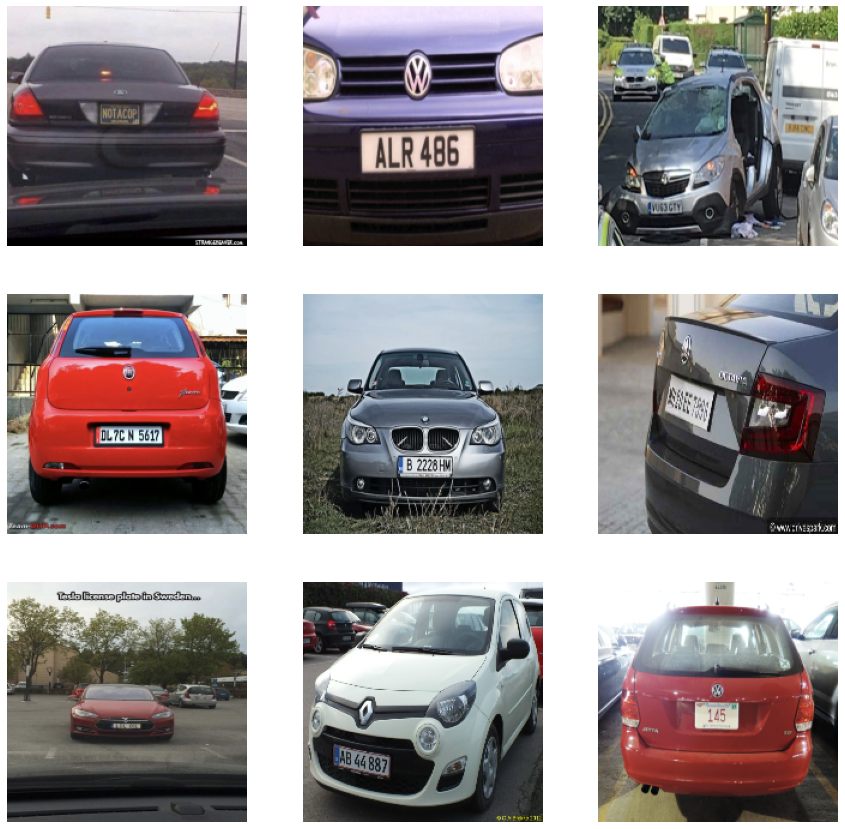
\includegraphics[width=\textwidth]{images/image_plate}
		\caption{Exemple des quelques images de notre dataset sans annotations }
		\label{fig:image_without_annotations}
	\end{figure}
	
	\begin{figure}[H]%bth
		\centering
		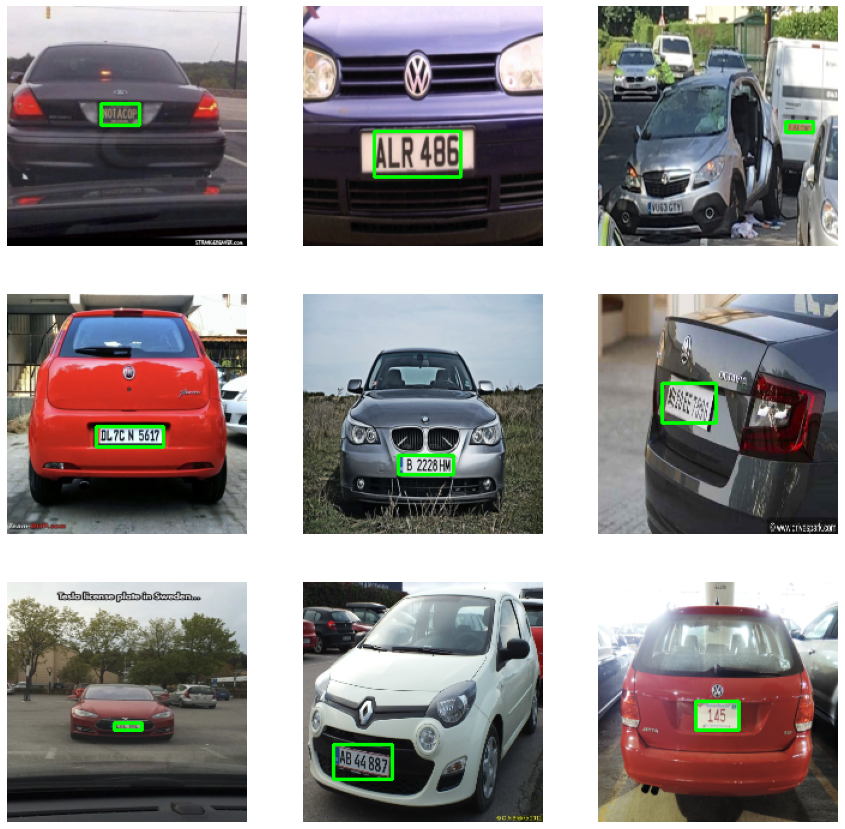
\includegraphics[width=\textwidth]{images/image_annotation}
		\caption{Exemple des images (figure \ref{fig:image_without_annotations}) de notre dataset sans annotations }
		\label{fig:image_with_annotations}
	\end{figure}

	\subsection{Entraînement  du CNN (VGG)}
	
	\subsubsection{Élaboration du modèle}
	\begin{table}[H]
	\begin{tabular}{|p{\textwidth}|}
		\hline
	\begin{lstlisting}[language=python]
import keras
from keras.models import Sequential, Model
from keras.layers import Dense, Flatten, Dropout
from keras.applications.vgg19 import VGG19
from keras.applications.vgg16 import VGG16
		
IMAGE_SIZE = 200
		
model = Sequential()

model.add(VGG16(
	weights="imagenet", 
	include_top=False, 
	input_shape=(IMAGE_SIZE, IMAGE_SIZE, 3))
)
model.add(Flatten())
model.add(Dropout(0.4))
model.add(Dense(256, activation="relu"))
model.add(Dense(128, activation="relu"))
model.add(Dense(64,  activation="relu"))
model.add(Dense(4,   activation="sigmoid"))
model.layers[-7].trainable = False

model.summary()
	\end{lstlisting}\\
		\hline
	\end{tabular}
	\end{table}
	
	
	Ci-dessus se trouve le code pour construire un modèle pré-entraîné VGG-16. Nous devons inclure { $weights = "imagenet"$} pour récupérer le modèle VGG-16 qui est formé sur l'ensemble de données imagenet. Il est important de définir $include\_top = False$ pour éviter de télécharger les couches entièrement connectées du modèle pré-entraîné \cite{tammina2019transfer}. Nous devons ajouter notre propre classificateur car le classificateur de modèle pré-entraîné a plus de 1 classe alors que notre objectif est de classer l'image en 1 classe (image de plaques). Une fois que les couches convolutionnelles du modèle pré-entraîné ont extrait les caractéristiques d'image de bas niveau telles que les bords, les lignes et les blobs, la couche entièrement connectée les classe ensuite en 1 catégories.
	
	Nous avons crée un modèle \textbf{"Séquentiel"} et ajoutons \textbf{VGG16} comme première couche. Le modèle prendra en entrée des tableaux de taille $( 200 \times 200 \times 3)$ qui correspondent à la taille d’une image du dataset. La sortie du VGG16 passe dans \textbf{Flatten} une couche qui a aplatis le tableau $( 200 \times 200 \times 3)$ en un tableau de taille $(18432 \times 1)$. Enfin nous ajoutons 4 couches \textbf{Dense} qui feront office d’un réseau complètement connecté avec comme sortie un tableau de taille $(4 \times 1)$ qui correspond au 4 points qui nous permettront d’obtenir ue rectangle contenant la plaque d'immatriculation sur l’image. 
	
	Ci-dessous le message de sortie, les informations sur notre reseaux de neurones construit.
	\begin{table}[H]
		\centering
		\begin{tabular}{lll}
			\hline
			Layer (type) & Output Shape & Param \# \\
			\hline
			\hline
			%& & \\
			\texttt{vgg16 (Functional) } &  \texttt{(None, 6, 6, 512) } & \texttt{14714688} \\
			
			\texttt{flatten (Flatten)}  & \texttt{(None, 18432)} & \texttt{0} \\ 
			
			\texttt{dropout (Dropout)} & \texttt{(None, 18432)} & \texttt{0} \\ 
			
			\texttt{dense (Dense)} & \texttt{(None, 256)} & \texttt{4718848 }\\
			
			\texttt{dense\_1 (Dense)} & \texttt{(None, 128)} & \texttt{32896} \\
			
			\texttt{dense\_2 (Dense)} & \texttt{(None, 64)} & \texttt{8256} \\ 
			
			\texttt{dense\_3 (Dense)} & \texttt{(None, 4)} & \texttt{260}  \\
			\hline
			\hline
			\multicolumn{3}{l}{
				\begin{tabular}{l}
					\texttt{Total params: 19,474,948} \\
					\texttt {Trainable params: 4,760,260} \\
					\texttt {Non-trainable params: 14,714,688} \\
				\end{tabular}
			}\\
			\hline
			
		\end{tabular}
	\end{table}


	Il est difficile de trouver un critère général pour arrêter cet algorithme. Le problème est que l'erreur tend à diminuer lentement et à ne jamais se stabiliser complètement, ce qui mène à un surapprentissage. La meilleure manière d'éviter ce phénomène est d'utiliser un ensemble de validation.

	%adam_loss_curve_3
	
	\begin{figure}[H]
		\myfloatalign
		\subfloat[loss : perte]
		{\label{fig:adam_loss_curve}
			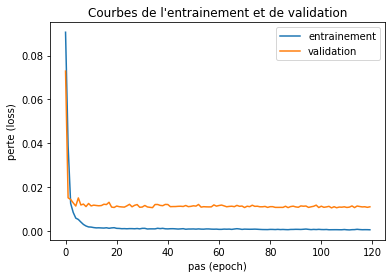
\includegraphics[width=.45\linewidth]{images/adam_loss_curve_3}} \quad
		\subfloat[accuracy : précision]
		{\label{fig:adam_accuracy_curve}
			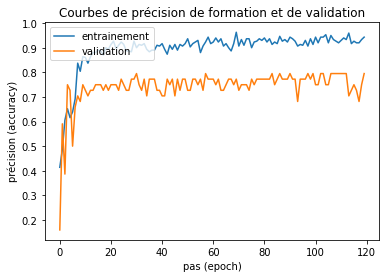
\includegraphics[width=.45\linewidth]{images/adam_accuracy_curve_3}} 
		
		\caption[]{Graphe de précision (accuracy) et perte (loss) du modèle VGG}\label{fig:adam_curve}
	\end{figure}
	Le script ci-dessous est une partie du programme que nous avons élaboré pour l'entraînement du CNN. Ici nous entraînons avec l'optimiseur SGD et un taux d'apprentissage de $1e-4 = 1.10^{-4}$. Dans la section \ref{sec:result_optimizer} nous montrons les résultats avec différents optimiseurs.
	
\begin{table}[H]
\begin{tabular}{|p{\textwidth}|}
	\hline
	\begin{lstlisting}[language=python]
import keras.optimizers as optimizers
import keras.losses as losses
optimizer = optimizers.SGD(learning_rate=1e-4)
loss = losses.MeanSquaredError(reduction="auto", name="mean_squared_error")
model.compile(loss=loss, optimizer=optimizer, metrics=['accuracy'])
model.fit(X_train, y_train, 
	validation_data=(X_val, y_val), 
	epochs=200, 
	batch_size=32, 
	verbose=1
)
	\end{lstlisting}\\
	\hline
\end{tabular}
\end{table}


\section{Évaluation du  résultats d'expérimentation}

	\subsection{Résultat comparatif des différent optimiseurs} \label{sec:result_optimizer}	

	Pour le même modèle élaboré pour la reconnaissance de plaque d'immatriculation. Nous allons tester son efficacité après entraînement en fonction des différents optimiseurs. Nous évaluons les quelques optimiseurs candidats pour cette études  (\cf $ \ $ chapitre \ref{chap:methode}, section \ref{sec:sgd_optimizers}). Voici une liste non exhaustive des optimiseurs étudiés.
	\subsubsection*{\qquad \textbullet \ SGD }
		\begin{table}[H]
			\centering
			\begin{tabular}{l|l|l}
				\hline
				\textbf{Training} & \textbf{Validation} & \textbf{Test} \\
				%& & \\
				\hline
				
				\texttt{loss: 0.0124} & \texttt{val loss: 0.0156} & \texttt{test loss: 0.0092} \\
				\texttt{accuracy: 0.6291} & \texttt{val accuracy: 0.6591} & \texttt{test accuracy: 0.5946} \\
				
				\hline
				
			\end{tabular}
		\end{table}
	
		\begin{figure}[H]
			\myfloatalign
			\subfloat[loss : perte]
			{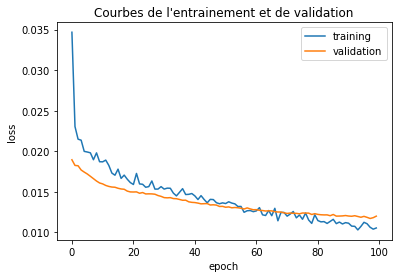
\includegraphics[width=.45\linewidth]{images/sgd_loss_curve}} \quad
			\subfloat[accuracy : précision]
			{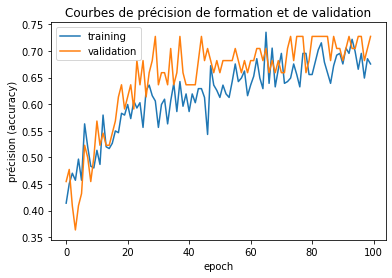
\includegraphics[width=.45\linewidth]{images/sgd_accuracy_curve}} 
			
			\caption[]{Graphe de précision (accuracy) et perte (loss)  pour RMSprop}
		\end{figure}
	\subsubsection*{\qquad \textbullet \ RMSprop}
		\begin{table}[H]
			\centering
			\begin{tabular}{l|l|l}
				\hline
				\textbf{Training} & \textbf{Validation} & \textbf{Test} \\
				%& & \\
				\hline

				\texttt{loss: 7.0379e-04} & \texttt{val loss: 0.0109} & \texttt{test loss : 0.005158} \\
				\texttt{accuracy: 0.9470} & \texttt{val accuracy: 0.7727} & \texttt{test accuracy : 0.86206} \\
				
				\hline
				
			\end{tabular}
		\end{table}
		\begin{figure}[H]
			\myfloatalign
			\subfloat[loss : perte]
			{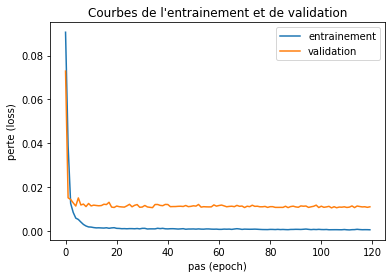
\includegraphics[width=.45\linewidth]{images/adam_loss_curve_3}} \quad
			\subfloat[accuracy : précision]
			{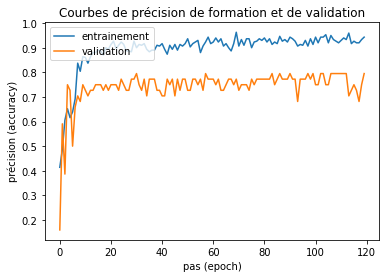
\includegraphics[width=.45\linewidth]{images/adam_accuracy_curve_3}} 
			
			\caption[]{Graphe de précision (accuracy) et perte (loss)  pour RMSprop}
		\end{figure}

	\subsubsection*{\qquad \textbullet \ Adagrad}
		\begin{table}[H]
			\centering
			\begin{tabular}{l|l|l}
				\hline
				\textbf{Training} & \textbf{Validation} & \textbf{Test} \\
				%& & \\
				\hline

				\texttt{loss: 0.0124} & \texttt{val loss: 0.0156} & \texttt{test loss: 0.0092} \\
				\texttt{accuracy: 0.6291} & \texttt{val accuracy: 0.6591} & \texttt{test accuracy: 0.5946} \\
				
				\hline
				
			\end{tabular}
		\end{table}
		\begin{figure}[H]
			\myfloatalign
			\subfloat[loss : perte]
			{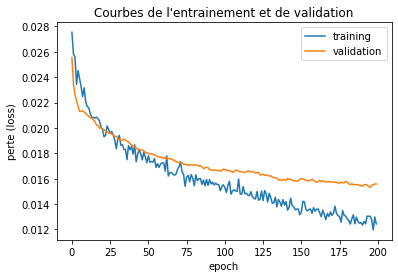
\includegraphics[width=.45\linewidth]{images/adagrad_loss_curve}} \quad
			\subfloat[accuracy : précision]
			{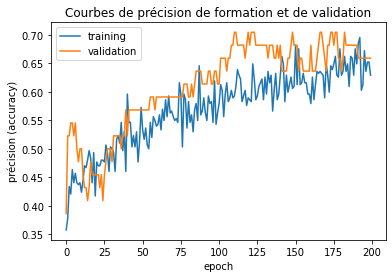
\includegraphics[width=.45\linewidth]{images/adagrad_accuracy_curve.png}} 
			
			\caption[]{Graphe de précision (accuracy) et perte (loss)  pour Adagrad}
		\end{figure}
	\subsubsection*{\qquad \textbullet \ Adadelta}
		\begin{table}[H]
			\centering
			\begin{tabular}{l|l|l}
				\hline
				\textbf{Training} & \textbf{Validation} & \textbf{Test} \\
				%& & \\
				\hline

				\texttt{loss: 0.0130} & \texttt{val loss: 0.0156} & \texttt{test loss : 0.01374378} \\
				\texttt{accuracy: 0.6523} & \texttt{val accuracy: 0.6591} & \texttt{test accuracy : 0.54022} \\
				
				\hline
				
			\end{tabular}
		
			\begin{figure}[H]
				\myfloatalign
				\subfloat[loss : perte]
				{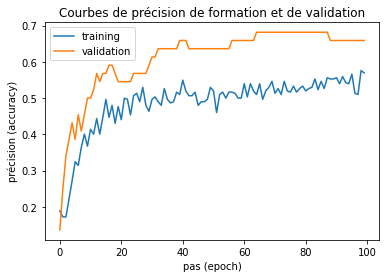
\includegraphics[width=.45\linewidth]{images/adadelta_accuracy_curve}} \quad
				\subfloat[accuracy : précision]
				{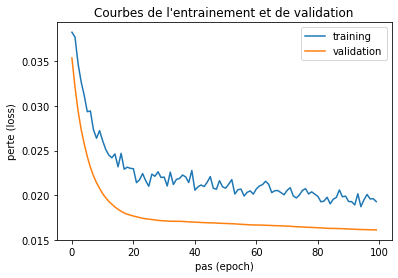
\includegraphics[width=.45\linewidth]{images/adadelta_loss_curve}} 
				
				\caption[]{Graphe de précision (accuracy) et perte (loss)  pour Adadelta}
			\end{figure}
		\end{table}
	\subsubsection*{\qquad \textbullet \ Adam}
		\begin{table}[H]
			\centering
			\begin{tabular}{l|l|l}
				\hline
				\textbf{Training} & \textbf{Validation} & \textbf{Test} \\
				%& & \\
				\hline

				\texttt{loss: 4.0037e-04} & \texttt{val loss: 0.0109} & \texttt{test loss : 0.00407} \\
				\texttt{accuracy: 0.9636} & \texttt{val accuracy: 0.7727} & \texttt{test accuracy : 0.88505} \\
				
				\hline
				
			\end{tabular}
		\end{table}
		\begin{figure}[H]
			\myfloatalign
			\subfloat[loss : perte]
			{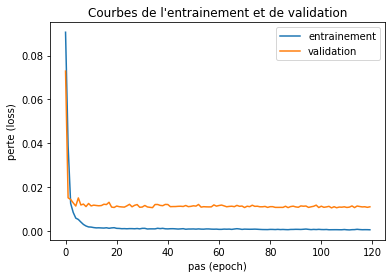
\includegraphics[width=.45\linewidth]{images/adam_loss_curve_3}} \quad
			\subfloat[accuracy : précision]
			{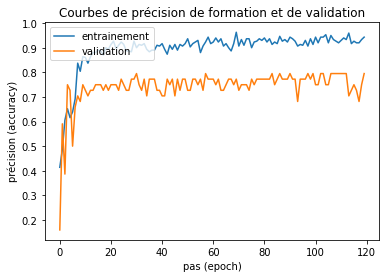
\includegraphics[width=.45\linewidth]{images/adam_accuracy_curve_3}} 
			
			\caption[]{Graphe de précision (accuracy) et perte (loss)  pour Adam}
		\end{figure}
		
	\subsubsection*{\qquad \textbullet \ Nadam}
	
		\begin{table}[H]
			\centering
			\begin{tabular}{l|l|l}
				\hline
				\textbf{Training} & \textbf{Validation} & \textbf{Test} \\
				%& & \\
				\hline
				\texttt{loss: 3.0496e-04} & \texttt{val loss: 0.0111} & \texttt{test loss : 0.004073061} \\
				\texttt{accuracy: 0.9536} & \texttt{val accuracy: 0.7955 }& \texttt{test accuracy : 0.87356}\\
				
				\hline 
				
			\end{tabular}
		\end{table}
	
		\begin{figure}[H]
			\myfloatalign
			\subfloat[loss : perte]
			{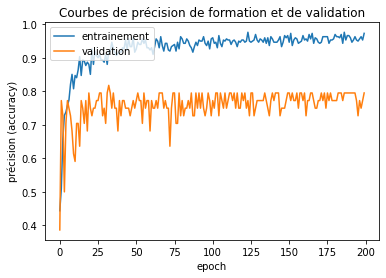
\includegraphics[width=.45\linewidth]{images/nadam_accuracy_curve}} \quad
			\subfloat[accuracy : précision]
			{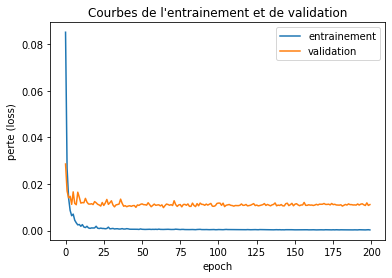
\includegraphics[width=.45\linewidth]{images/nadam_loss_curve}} 
			
			\caption[]{Graphe de précision (accuracy) et perte (loss)  pour Nadam}
		\end{figure}
	
	
	%Efficacité du modèle par rapport au critère de l'invariance des transformation géométrique\
	
	Nous remarquons RMSprop minimise le mieux les erreurs par rapport aux autres optimiseurs mais il n’est pas précis par rapport à Nadam ou Adam. Ci-dessous une liste des optimiseurs qui minimise le mieux dans le cas de notre problème reconnaissance de plaque d’immatriculation.
	
	\begin{table}[H]
		\centering
		\begin{tabular}{|l|p{3cm}|p{3cm}|p{3cm}|}
			\hline
			\textbf{N\textdegree} & \textbf{Training} & \textbf{Validation} & \textbf{Test} \\
			\hline
			\textbf{1. RMSprop} &
			\texttt{7.0379e-04} &
			\texttt{0.0109} &
			\texttt{0.005158} \\
			\hline
			\textbf{2. Nadam} &
			\texttt{3.0496e-04} &
			\texttt{0.0111} &
			\texttt{0.004073} \\
			\hline
			\textbf{3. Adam} &
			\texttt{4.0037e-04} &
			\texttt{0.0109} &
			\texttt{0.00407} \\
			\hline
			\textbf{4. Adagrad} &
			\texttt{0.0124} &
			\texttt{0.0156} &
			\texttt{0.0092} \\
			\hline
			\textbf{5. Adadelta} &
			\texttt{0.0130} &
			\texttt{0.0156} &
			\texttt{0.013743} \\
			\hline
		\end{tabular}
	\end{table}
	
	
	
	\subsection{Invariance des transformation géométrique}
	%\cite{deepa2021ai,ahadjitse2013reconnaissance}\cite{amari1993backpropagation}. 
	%parler de l'invariance à la transformations
	
	%Pour notre
	
	%???
	
	%\lipsum[4]

	
	%\subsection{Évaluation du résultats de l'expérimentation}
	%\subsubsection{Utiliser le modèle formé pour faire des prédictions}
	%\lipsum[1] 
	%\subsubsection{Problèmes posés}
	
	Nous avons dit en amont que le modèle entraîné doit reconnaître les objet même après transformation géométrique dans l’image. Nous allons examiner l'efficacité par rapport au 3 meilleur optimiseurs c.a.d les 3 modèle qui ont on eu un bon score d'entraînement, de validation et de test.
	
	
	\begin{table}[H]
		\centering
		\begin{tabular}{l|r|r|r}
			\hline
			 & \textbf{Training} & \textbf{Validation} & \textbf{Test} \\
			
			\hline
			\textbf{Nadam} &
			\texttt{95.36\%} &
			\texttt{79.55\%} &
			\texttt{87.35\%} \\
			\hline
			\textbf{Adam} &
			\texttt{96.36\%} &
			\texttt{77.27\%} &
			\texttt{88.50\%} \\
			\hline
			\textbf{RMSprop} &
			\texttt{94.70\%} &
			\texttt{77.27\%} &
			\texttt{86.20\%} \\
			\hline
			
		\end{tabular}
	\end{table}
	
	??? (Suite)	
	
	%\section{Défis \& problèmes rencontrés}
	
	%Les données sont pas disponibles cas du dataset, 
	%\subsection{Cas du gradient bloqué}
	%cas du gradient bloqué
	
	
	
	%???
	
	\section{Sommaire du chapitre}
	C’est là toute la force des réseaux de neurones convolutifs : ceux-ci sont capables de déterminer tout seul les éléments discriminants d'une image, en s'adaptant au problème posé. Par exemple, si la question est de distinguer les chats des chiens, les features automatiquement définies peuvent décrire la forme des oreilles ou des pattes. 
	

